%%%%%%%%%%%%%%%%%%%%%%%%%%%%%%%%%%%%%%
  %%%%%%%%%%%%%%%%%%%%%%%%%%%%%%%%%%%%%%
  % Do not edit the TeX file your work
% will be overwritten.  Edit the RnW
% file instead.
%%%%%%%%%%%%%%%%%%%%%%%%%%%%%%%%%%%%%%
  %%%%%%%%%%%%%%%%%%%%%%%%%%%%%%%%%%%%%%
  
  
      
      
      

\begin{knitrout}
\definecolor{shadecolor}{rgb}{0.969, 0.969, 0.969}\color{fgcolor}\begin{figure}[!h]

{\centering 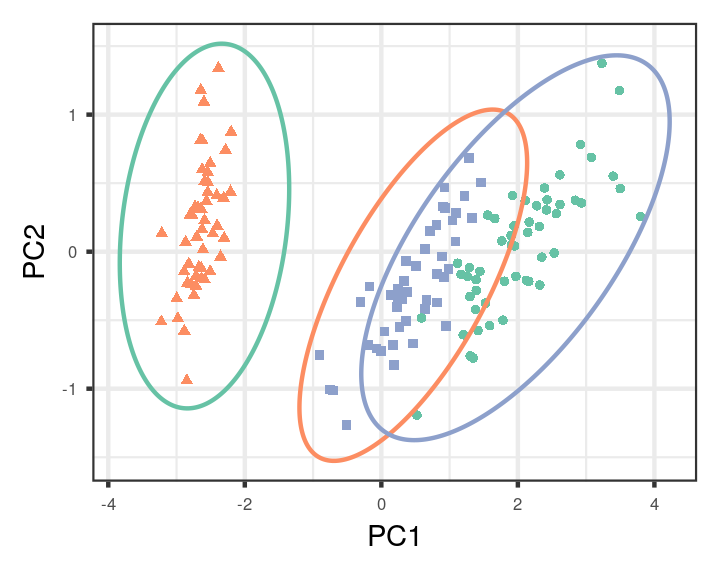
\includegraphics[width=0.98\linewidth,height=0.784\linewidth]{figure/iris_fit-1} 

}

\caption[The iris fit]{The iris fit.  }\label{fig:iris_fit}
\end{figure}


\end{knitrout}



\begin{knitrout}
\definecolor{shadecolor}{rgb}{0.969, 0.969, 0.969}\color{fgcolor}\begin{figure}[!h]

{\centering 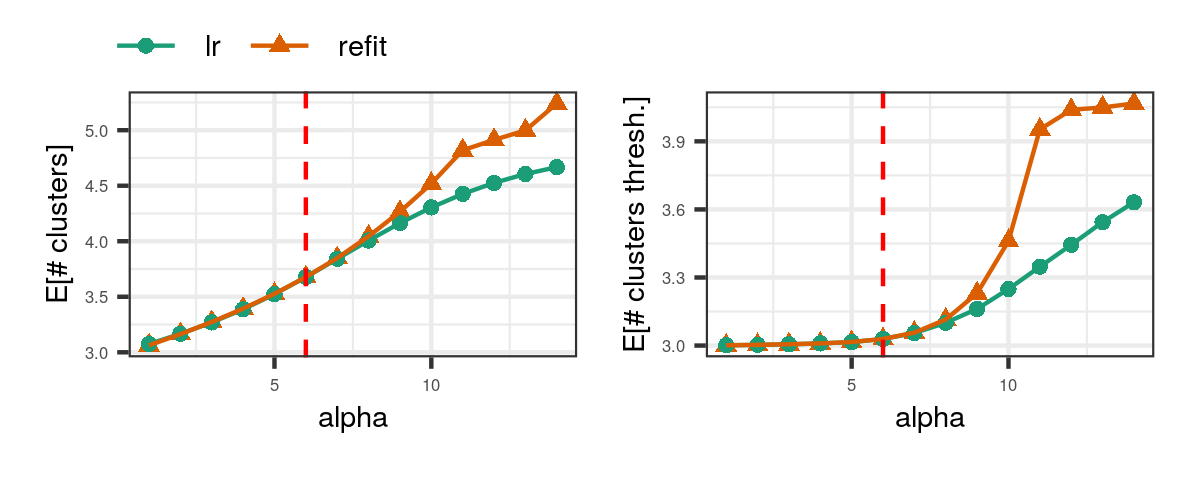
\includegraphics[width=0.98\linewidth,height=0.392\linewidth]{figure/iris_alpha_sens-1} 

}

\caption[iris alpha sensitivity ]{iris alpha sensitivity }\label{fig:iris_alpha_sens}
\end{figure}


\end{knitrout}



\begin{knitrout}
\definecolor{shadecolor}{rgb}{0.969, 0.969, 0.969}\color{fgcolor}\begin{figure}[!h]

{\centering 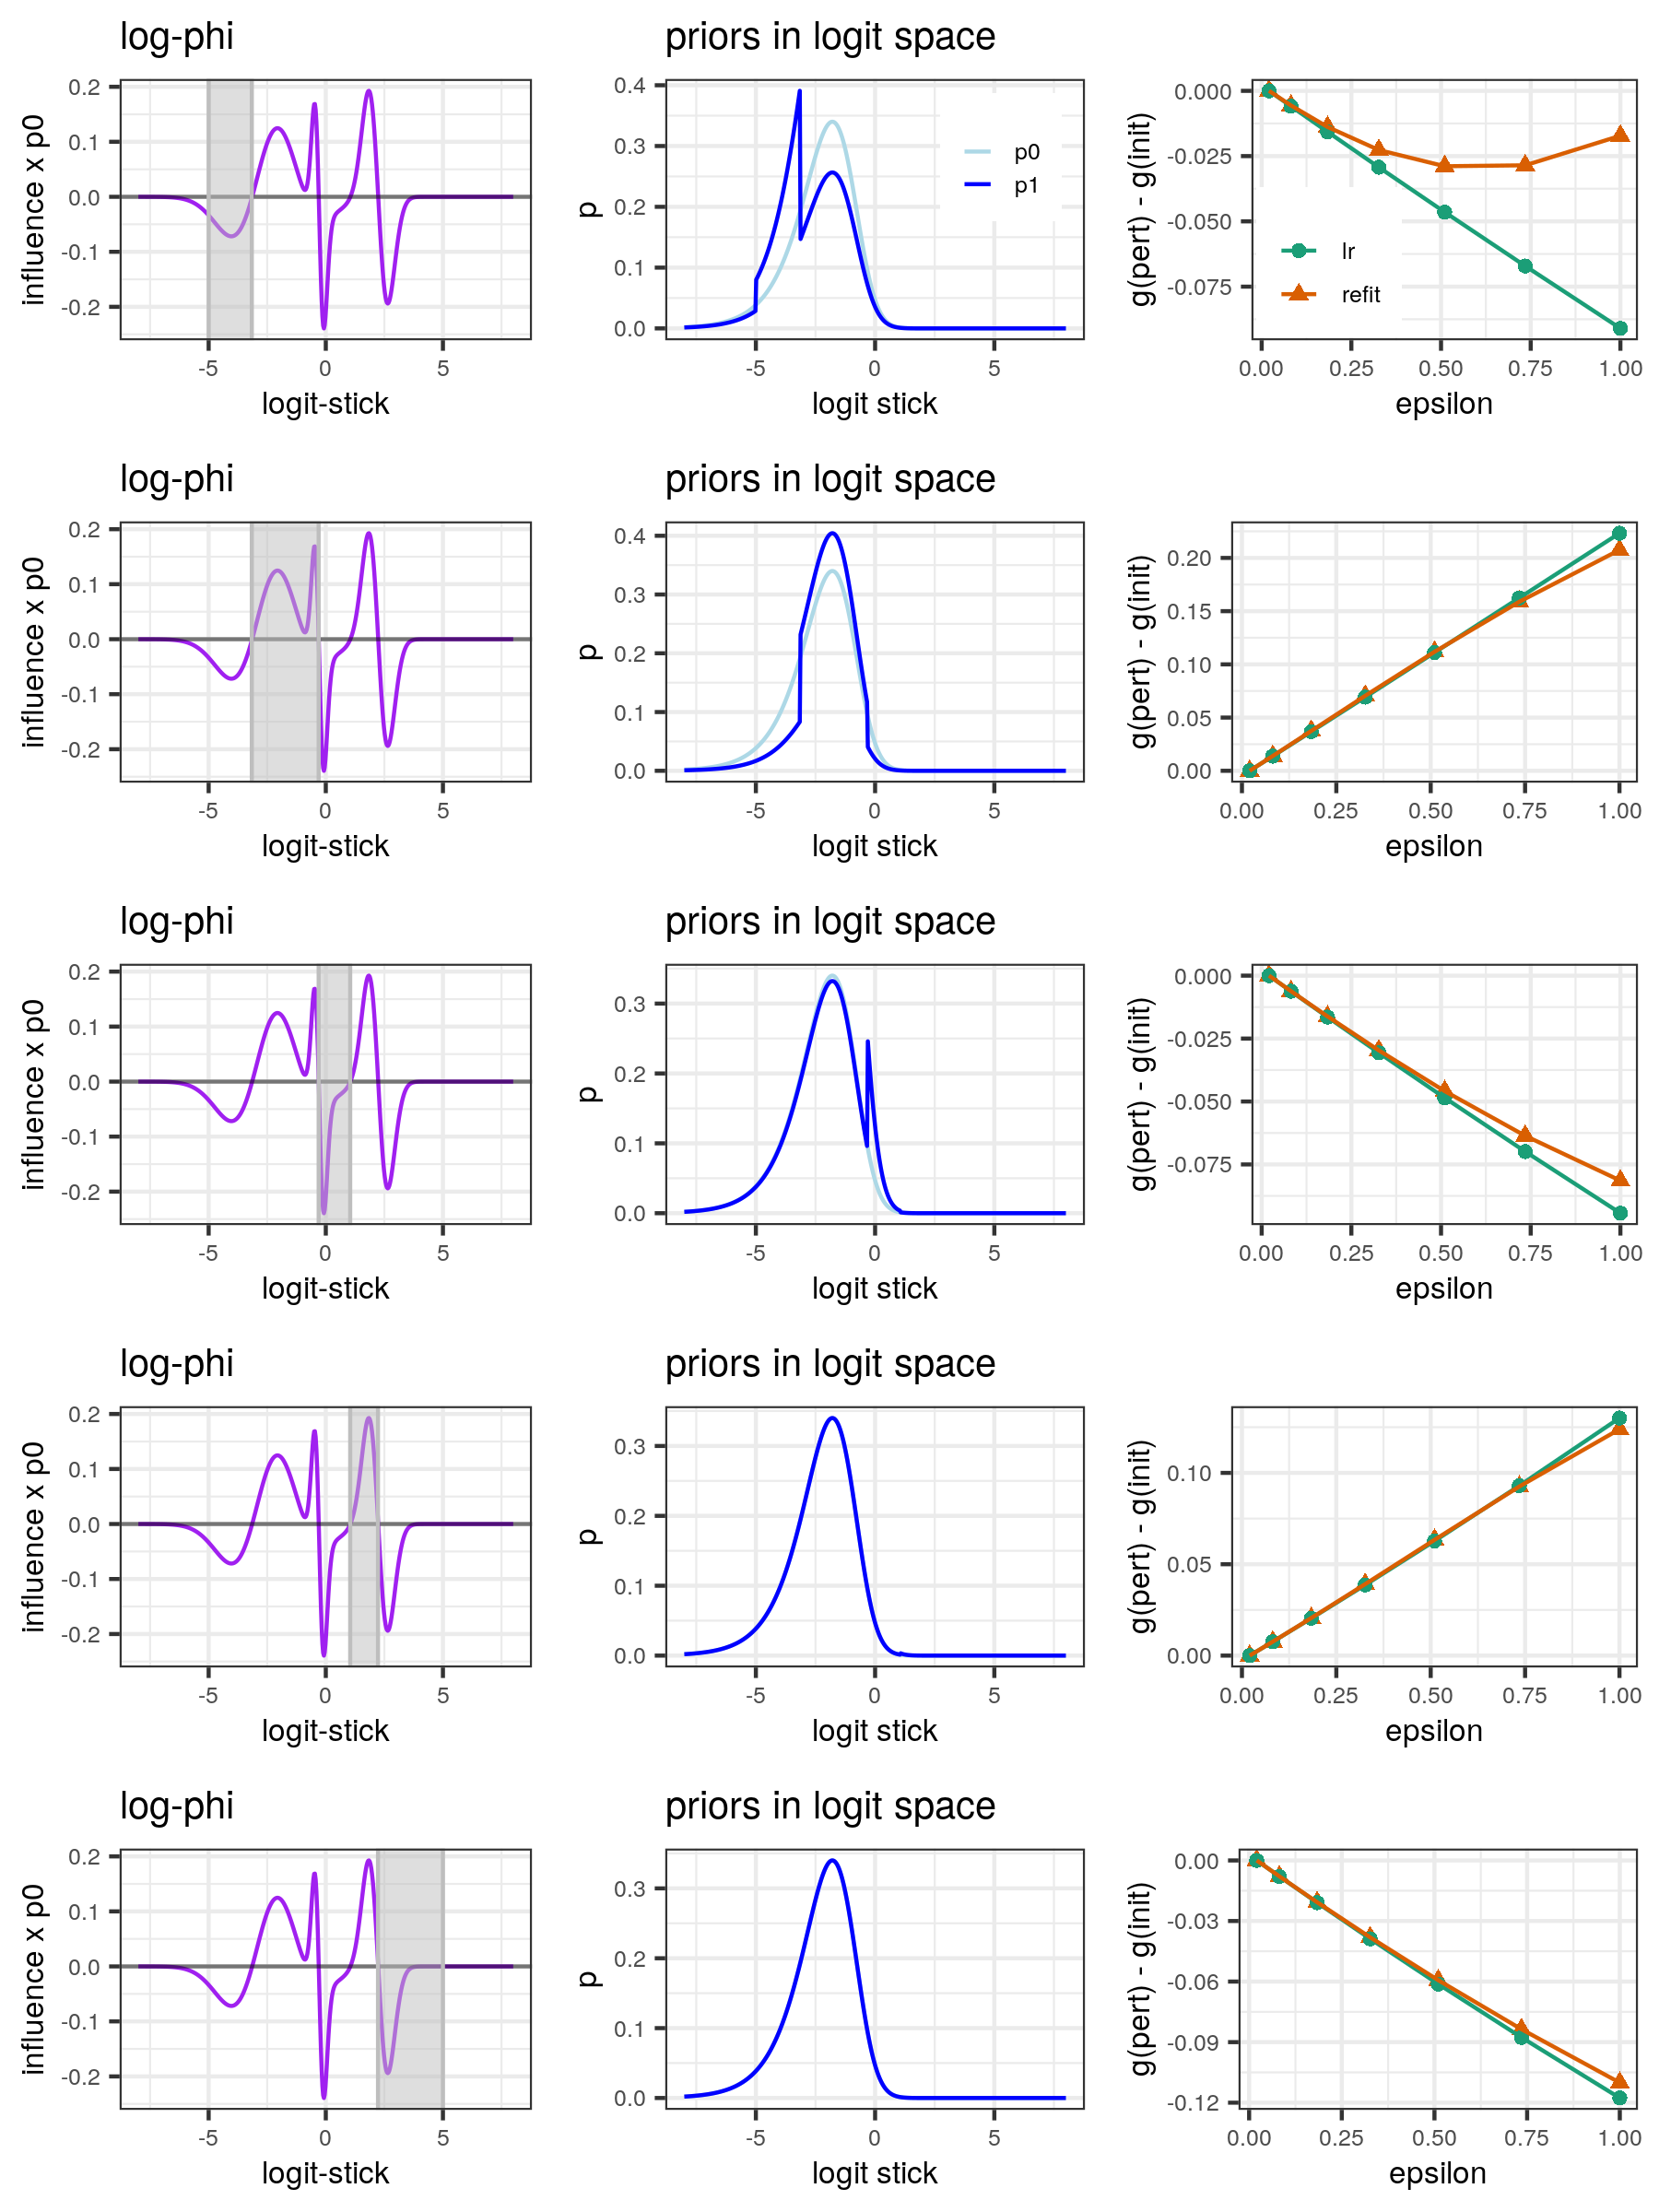
\includegraphics[width=0.98\linewidth,height=1.098\linewidth]{./R_scripts/iris/figures_tmp/iris_func_pert} 

}

\caption[iris functional sensitivity ]{iris functional sensitivity }\label{fig:iris_fsens}
\end{figure}


\end{knitrout}


